% Paquets g�n�raux
\documentclass[a4paper,12pt,titlepage]{article}

%%%%%%%%%%%%%%%%%%%%%%%%%%%%%%%%%%%%%%%%%
%%%%%%%%%%%%Partie � modifier%%%%%%%%%%%%
\newcommand{\theme}{Statique, lois de Coulomb}
\newcommand{\sujet}{Mod�liser le comportement statique de syst�mes avec frottement}
\newcommand{\objectifs}{D�couverte de l'arc-bouttement\\
Mise en �vidence de l'influence des efforts r�partis}
%Si un seul support 0
\newcommand{\nbsupport}{0}
\newcommand{\supportu}{Cordeuse}
\newcommand{\supportimageu}{img/cordeuse}
%%%%%%%%%%%%%%%%%%%%%%%%%%%%%%%%%%%%%%%%%
\usepackage[T1]{fontenc}
\usepackage[latin9]{inputenc}
\usepackage[french]{babel}
\usepackage[gen]{eurosym}
%\usepackage[dvips]{graphicx}
\usepackage{fancyhdr}
\usepackage{pdfpages} 
\usepackage{multido}
\usepackage{vmargin}
%\usepackage{aeguill}
\usepackage{color}
\usepackage{xcolor}
\usepackage{helvet}
\renewcommand{\familydefault}{\sfdefault}
\usepackage{amsfonts}
\usepackage{amsmath}
%\usepackage{xspace}
\usepackage{varioref}
\usepackage{tabularx}
%\usepackage{floatflt}
\usepackage{graphics}
%\usepackage{wrapfig}
\usepackage{textcomp}
%\usepackage{boxedminipage}
\definecolor{forestgreen}{rgb}{0.13,0.54,0.13}
\definecolor{blcr}{rgb}{0.59,0.69,0.84}
\definecolor{blfr}{rgb}{0.32,0.51,0.75}
\definecolor{orfr}{rgb}{0.90,0.42,0.15}
\definecolor{orcr}{rgb}{0.90,0.65,0.50}
\definecolor{orangef}{rgb}{0.659,0.269,0.072}
\definecolor{orange}{rgb}{0.58,0.35,0.063}
\definecolor{orangec}{rgb}{0.43,0.32,0.25}
\definecolor{rcorrect}{rgb}{0.6,0,0}

% Mise en page
\pagestyle{fancy}

\setlength{\hoffset}{-18pt}

\setlength{\oddsidemargin}{0pt} 	% Marge gauche sur pages impaire2s
\setlength{\evensidemargin}{0pt} 	% Marge gauche sur pages paires
\setlength{\marginparwidth}{00pt} 	% Largeur de note dans la marge
\setlength{\headwidth}{481pt} 	 	% Largeur de la zone de t�te (17cm)
\setlength{\textwidth}{481pt} 	 	% Largeur de la zone de texte (17cm)
\setlength{\voffset}{-18pt} 		% Bon pour DOS
\setlength{\marginparsep}{7pt}	 	% S�paration de la marge
\setlength{\topmargin}{-30pt} 		% Pas de marge en haut
\setlength{\headheight}{55pt} 		% Haut de page
\setlength{\headsep}{20pt} 			% Entre le haut de page et le texte
\setlength{\footskip}{30pt} 		% Bas de page + s�paration
\setlength{\textheight}{700pt} 		% Hauteur de la zone de texte (25cm)
\setlength\fboxrule{1 pt}
\renewcommand{\baselinestretch}{1}
\setcounter{tocdepth}{1}
\newcommand{\cadre}[2]
{\fbox{
  \begin{minipage}{#1\linewidth}
   \begin{center}
    #2\\
   \end{center}
  \end{minipage}
 }
}

\newcommand{\reponse}[1][4]
{
\multido{}{#1}
{\centering\makebox[0.9\linewidth]{}  \\
\centering\makebox[0.9\linewidth]{\dotfill} \\
}}

\newcommand{\titre}[1]
{\begin{center}
\cadre{0.8}{\huge #1} 
\end{center}
}

% En t�te et pied de page
\lhead{\theme}
\rhead{\includegraphics[width=2cm]{../../../Admin/Logo_Corbu.PNG}}
\lfoot{Renaud Costadoat}
\cfoot{Page \thepage}

\fancypagestyle{correction}{%
  \fancyhf{}
  \lhead{\colorbox{rcorrect}{\begin{minipage}{0.65\paperwidth} \textcolor{white}{\textbf{Correction}} \end{minipage}} }
  \rhead{\includegraphics[width=2cm]{../../../Admin/Logo_Corbu.PNG}}
  \lfoot{Renaud Costadoat}
  \rfoot{\colorbox{rcorrect}{\begin{minipage}{0.6\paperwidth} \begin{flushright}\textcolor{white}{\textbf{Correction}}\end{flushright} \end{minipage}} }}

\renewcommand{\footrulewidth}{0.4pt}

\begin{document}
\pagestyle{empty}
\setlength{\headheight}{0pt}
\setlength{\footskip}{0pt}


\hspace{-2cm}\colorbox{blcr}{\begin{minipage}{0.95\paperwidth}
\begin{minipage}{0.7\linewidth}
\vspace{5pt} \large \textbf{CPGE PTSI} \\ \vfill
Sciences Industrielles pour l'Ing�nieur \\ \vfill
Renaud Costadoat \vspace{5pt}
\end{minipage}
 \hfill 
\begin{minipage}{0.18\linewidth}
\begin{flushright}
Lyc�e le Corbusier\\ \vfill
\includegraphics[width=2cm]{../../../Admin/Logo_Corbu.PNG}
\end{flushright}
\end{minipage}\end{minipage}}

\hspace{-2cm}\colorbox{blfr}{\begin{minipage}{0.95\paperwidth}
\Large\textcolor{white}{\\\textbf{Compte rendu} \hfill \textbf{\theme} \hfill \textit{Date:} .../.../...... 
}\end{minipage}} 

\vspace{1cm}
\begin{center}
\colorbox{forestgreen}{\begin{minipage}{0.9\linewidth}\textcolor{white}{\large\textit{Th�me:} \\ \sujet} \end{minipage}}\\
\colorbox{orfr}{\begin{minipage}{0.9\linewidth}\large\textit{Objectifs:} \\ \objectifs \end{minipage}} \\
\colorbox{orcr}{\begin{minipage}{0.9\linewidth}\large\textit{Support:}   \\ \Huge\textsf{\supportu} \\ \begin{center}\includegraphics[width=0.7\linewidth]{\supportimageu}\end{center} \vspace{10pt} \end{minipage}} \\ \vspace{40pt}
\end{center}



\colorbox{blcr}{\large\begin{minipage}{0.45\linewidth}Nom:.................................\end{minipage}}
\colorbox{blcr}{\large\begin{minipage}{0.45\linewidth}Pr�nom:.................................\end{minipage}}

\colorbox{blcr}{\large\begin{minipage}{0.45\linewidth}Nom:.................................\end{minipage}}
\colorbox{blcr}{\large\begin{minipage}{0.45\linewidth}Pr�nom:.................................\end{minipage}}

\colorbox{blcr}{\large\begin{minipage}{0.45\linewidth}Nom:.................................\end{minipage}}
\colorbox{blcr}{\large\begin{minipage}{0.45\linewidth}Pr�nom:.................................\end{minipage}}

\newpage

\setlength{\headheight}{55pt}
\setlength{\footskip}{30pt} 
\setlength{\textheight}{700pt} 	
\pagestyle{fancy}

%%%%%%%%%%%%%%%%%%%%%%%%%%%%%%%%%%%%%%%%%%%%%%%%%%%%%%%%%%%%%%%%%%%%%%%%%%%%%%%%%%%%%%%%%%%%%%%%%%%%%%%%%%%%%%%%%%%%
%%%%%%%%%%%%%%%%%%%%%%%%%%%%%%%%%%%%%%%%%%%%%%%%%%%%%%%%%%%%%%%%%%%%%%%%%%%%%%%%%%%%%%%%%%%%%%%%%%%%%%%%%%%%%%%%%%%%


\section{La Cordeuse}

\subsection{Fonctionnement du syst�me}

\begin{figure}[!h]
 \begin{minipage}{0.45\linewidth}
L'objectif de cette �tude est l'�tude du comportement de la liaison glissi�re qui guide le d�placement de la pince.

Une fois le syst�me mis en route et apr�s avoir analys� son fonctionnement, effectuer la manipulation propos�e sur le diaporama de la cordeuse. 
 \end{minipage}
  \hfill
 \begin{minipage}{0.45\linewidth}
  \centering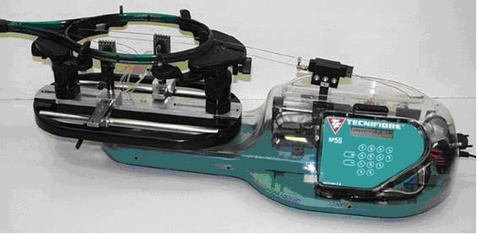
\includegraphics[width=0.7\linewidth]{img/cordeuse.png}
  \caption{Syst�me Maxpid}
  \label{img1}
 \end{minipage}
\end{figure}

\paragraph{Question 1:} Que constatez-vous quant au comportement de la liaison glissi�re pince-berceau ? Satisfait-elle � la fonction \og bloquer le d�placement de la corde \fg. Une liaison parfaite pourrait-elle convenir ? En manipulant � la main la pince, expliquer ce qui conditionne le blocage de la liaison.

\reponse[2]

\subsection{Ph�nom�ne d'arc-bouttement}

\paragraph{Question 2:} Par une approche de statique graphique et analytique, d�terminez l?expression de $h_{limite}$ (en fonction de L, et j) au-del� de laquelle il y a blocage. Le blocage d�pend-t-il de l'intensit� de l'effort dans le ph�nom�ne d'arc-boutement ?

\reponse[3]

\subsection{Exp�rimentation sur la maquette de la glisi�re}

\paragraph{Question 3:} A partir de cette maquette, proposer un protocole exp�rimental qui permet de v�rifier en partie les r�sultats pr�c�dents.

Prendre toutes les hypoth�ses utiles pour effectuer cette exp�rimentation.

\reponse[3]

\end{document}
